\documentclass[12pt]{article}
\usepackage[utf8]{inputenc}
\usepackage{geometry}
\geometry{margin=1in}
\usepackage{amsmath}
\usepackage{tikz}
\usepackage{pgfplots}
\pgfplotsset{compat=1.15}

\title{Island Economy Exercise}
\author{Macroeconomics \\ Scarcity and Choice}
\date{}

\begin{document}
\maketitle

\section*{Part A: Scarcity and Trade-Offs (Round 1)}
\textbf{Decision Example (10 tokens):}
\begin{itemize}
    \item Fish Produced: 6
    \item Shelters Produced: 2
\end{itemize}

\noindent \textbf{Sample Answers:}
\begin{enumerate}
    \item The trade-off was between food (fish) and protection (shelters). More fish means fewer shelters, and vice versa.
    \item To produce 1 more shelter (cost = 2 tokens), the group must give up 2 fish. Opportunity cost of 1 shelter = 2 fish.
\end{enumerate}

\section*{Part B: Production Possibilities Frontier (PPF)}
\noindent \textbf{PPF Points with 10 Tokens:}
\[
\begin{aligned}
0 \text{ Shelters} &\to 10 \text{ Fish} \\
1 \text{ Shelter} &\to 8 \text{ Fish} \\
2 \text{ Shelters} &\to 6 \text{ Fish} \\
3 \text{ Shelters} &\to 4 \text{ Fish} \\
4 \text{ Shelters} &\to 2 \text{ Fish} \\
5 \text{ Shelters} &\to 0 \text{ Fish} \\
\end{aligned}
\]

\begin{center}
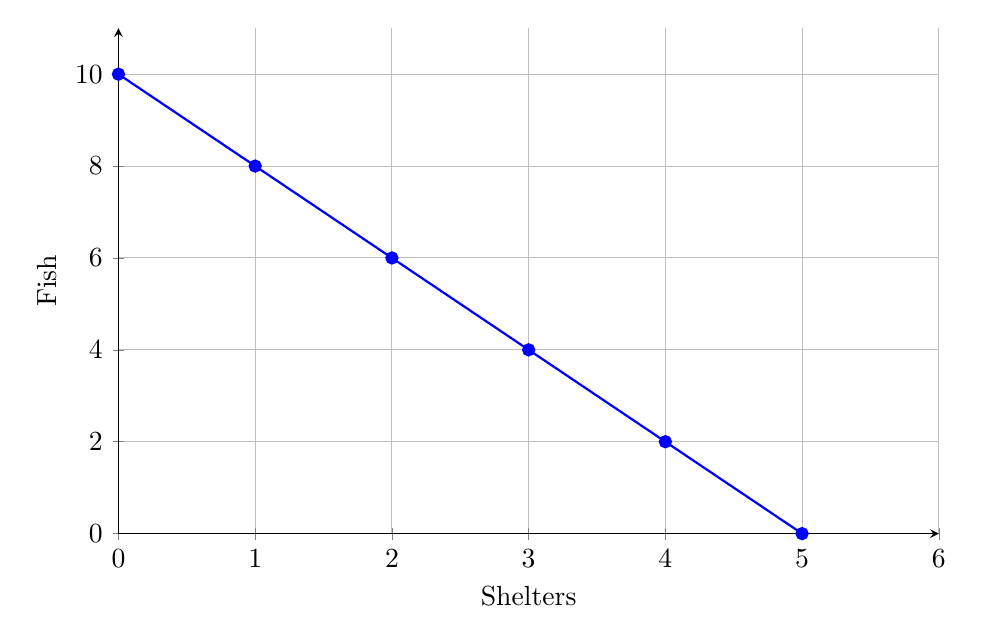
\begin{tikzpicture}
\begin{axis}[
    width=12cm, height=8cm,
    axis lines=left,
    xlabel={Shelters},
    ylabel={Fish},
    xmin=0, xmax=6,
    ymin=0, ymax=11,
    xtick={0,...,6},
    ytick={0,2,...,10},
    grid=both
]
% PPF points
\addplot[mark=*, thick, blue] coordinates {
    (0,10) (1,8) (2,6) (3,4) (4,2) (5,0)
};
\end{axis}
\end{tikzpicture}
\end{center}

\noindent \textbf{Note:} The PPF is linear in this setup because opportunity cost is constant (1 shelter = 2 fish).

\section*{Part C: Specialization and Trade (Round 2)}
\noindent Example:  
\begin{itemize}
    \item Group A (Fishing Advantage): 10 tokens $\to$ 20 Fish
    \item Group B (Shelter Advantage): 10 tokens $\to$ 10 Shelters
\end{itemize}

If they specialize and trade:  
- Suppose Group A trades 10 fish for 4 shelters with Group B.  
- Final Bundles:  
  - Group A: 10 Fish + 4 Shelters  
  - Group B: 10 Fish + 6 Shelters  

\noindent \textbf{Sample Answers:}
\begin{enumerate}
    \item Specialization increased total production: 20 fish + 10 shelters vs. mixed production with less output.
    \item Both groups are better off after trade compared to autarky (no trade).
\end{enumerate}

\section*{Part D: Economic Shocks (Round 3)}
\begin{enumerate}
    \item If a storm destroys half of all shelters, shelters become more valuable relative to fish. The opportunity cost of a shelter rises.
    \item A new fishing net doubling fishing productivity shifts the PPF outward in the fish direction. Now 1 token = 2 fish, so the maximum is 20 fish (with 0 shelters). The economy can consume more fish for any given number of shelters.
\end{enumerate}

\section*{Reflection Questions – Suggested Responses}
\begin{enumerate}
    \item Scarcity is shown because groups cannot produce unlimited amounts of both goods with only 10 tokens.
    \item The PPF shows opportunity costs: the slope represents how many fish must be given up for each shelter.
    \item Countries specialize and trade for the same reason as the groups — comparative advantage increases total production and allows everyone to be better off.
    \item When resources or technology change, the PPF shifts outward (growth) or inward (loss), changing the economy’s possible choices.
\end{enumerate}

\end{document}
